\documentclass[xcolor=svgnames]{beamer}
\usetheme[
    %%% options passed to the outer theme
    %    hidetitle,           % hide the (short) title in the sidebar
    %    hideauthor,          % hide the (short) author in the sidebar
    %    hideinstitute,       % hide the (short) institute in the bottom of the sidebar
    %    shownavsym,          % show the navigation symbols
         width=1.5cm,         % width of the sidebar (default is 2 cm)
    %    hideothersubsections,% hide all subsections but the subsections in the current section
    %    hideallsubsections,  % hide all subsections
         left                 % right of left position of sidebar (default is right)
    %%% options passed to the color theme
        lightheaderbg         % use a light header background
  ]{AAUsidebar}
\setbeameroption{show notes}

% #### graphics and schemes
\usepackage{graphicx}
\graphicspath{{img/}}
\usepackage{tikz}
\usetikzlibrary{                          % TikZ libraries
                scopes,                   % .
                shapes,                   % .
                arrows,                   % .
                through,                  % .
                calc,                     % .
                intersections,            % .
                spy,                      % .
                matrix,                   % .
                chains,                   % .
                mindmap,                  % .
                trees,                    % .
                decorations.pathreplacing,% .
                decorations.pathmorphing, % .
                decorations.markings}     % .

\usepackage{pgfplots}                     % TikZ plots
\usepackage{pgfplotstable}                % TikZ tables from CSV
\pgfplotsset{compat=1.3}                  % activates \xilabel shift` for pgfplots
\usepackage{array}
\usepackage{listings}
\usepackage{times}
\usepackage{amsmath}
\usepackage{verbatim}
\usepackage{ccicons}
\usepackage{tcolorbox}
\usepackage{chronosys}
\usepackage{listings}                     % code
\usepackage{adjustbox}                    % code
\usepackage{attrib}

% #### colors
\usepackage{xcolor}                       % common color names
\usepackage{colortbl}                     % common color names

% #### layouts
\usepackage{multicol}
\usepackage[textfont=footnotesize,bf]{caption}
\usepackage{subfig}

% #### fonts
\usepackage[utf8]{inputenc}
\usepackage[english]{babel}
\usepackage[T1]{fontenc}
\usepackage{cmbright}
\usepackage{soul} %slanted text
\usepackage{hyperref}
\urlstyle{same}
\hypersetup{pdfauthor={Francesco de Virgilio},pdftitle={HIRMEOS: a collaborative perspective on altmetrics for monographs}}

% #### tables
\usepackage{booktabs}			          % migliora la qualità delle tabelle
\usepackage{tabularx}			          % colonne a spaziatura fissa delle tabelle
\newcommand{\otoprule}                    % better top rule horizontal line
    {\midrule[\heavyrulewidth]}           % .


\begin{document}

\usebackgroundtemplate{
    
\includegraphics[width=\paperwidth,height=\paperheight]{img/cover}
}

    \begin{frame}[plain,noframenumbering]
        \begin{center}
            \color{RoyalBlue}
            \textbf{
                \Huge{HIRMEOS}\\
                \Large{A collaborative perspective on altmetrics for monographs}\\
            }
            \vspace{40pt}
            Francesco de Virgilio\\
            \vspace{8pt}
            \scriptsize{Tech Team Lead, Ubiquity Press}\\
            \scriptsize{Hamburg, 14/05/2018}
        \end{center}
    \end{frame}

\usebackgroundtemplate{%
    
\includegraphics[width=\paperwidth,height=\paperheight]{img/background}
}

\section{The company}

    \begin{frame}{Disclaimer(s)}
        \pause
        \begin{block}{Disclaimer 1}
            Techies? Non-techies? I will stay in the middle.
        \end{block}
        \pause
        \vspace{0.05\textheight}
        \begin{block}{Disclaimer 2}
            There are some good news at the end of this presentation.
        \end{block}
        \pause
        \vspace{0.05\textheight}
        \begin{block}{Disclaimer 3}
            No kittens, sorry.
        \end{block}
    \end{frame}

    \subsection{Mission}

        \begin{frame}{Bragging}
            \begin{center}
                \Huge{< Bragging >}
            \end{center}
        \end{frame}

        \begin{frame}{What's Ubiquity Press?}
            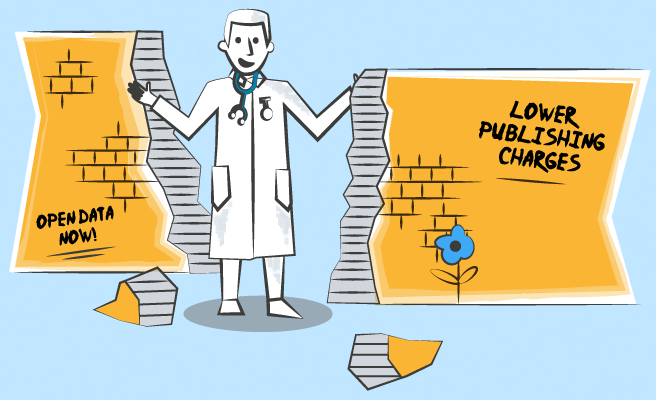
\includegraphics[width=0.7\textwidth]{img/up_banner}
            \begin{block}{Mission}
                To return control of publishing to universities, libraries, societies and researchers, providing them with the infrastructure and support to not only match but to outcompete the legacy publishers.
            \end{block}
        \end{frame}

    \subsection{Background}

        \begin{frame}{What's Ubiquity Press?}
            \begin{itemize}
                \item Spun out of University College London in 2012
                \item Researcher-led
                \item Grown out of the humanities
                \item 100+ years publishing experience
                \item Comprehensive approach: journals,
                \item books, data, software, wetware…
                \item Offices in London and Oakland
                \item Open access only
                \item we are interested in tech...
            \end{itemize}
        \end{frame}

        \begin{frame}{/Bragging}
            \begin{center}
                \Huge{< /Bragging >}
            \end{center}
        \end{frame}

\section{The project}

    \subsection{Definition}

        \begin{frame}{HIRMEOS}
            \begin{center}
                
\includegraphics[width=0.7\textwidth]{img/hirmeos}
                \color{black}
                \begin{block}{It's about monographies}
                    High Integration of Research Monographs in the European Open Science Infrastructure (Humanities and Social Sciences)
                \end{block}

                \pause

                \begin{itemize}
                    \item overcome technical limitations to publish open access monographs
                    \pause
                    \item enable collaboration between selected partners
                    \pause
                    \item release all software and tools as open source
                \end{itemize}
            \end{center}
        \end{frame}

        \begin{frame}{Who's involved}
            \begin{center}
                \begin{itemize}
                    \item Centre National de la Recherche Scientifique (CNRS) [FR]
                    \item Ethniko Idryma Erevnon (NHRF - EIE) [GR]
                    \item Stitching OAPEN (Open Access Publishing in European Networks) (OAPEN) [NL]
                    \item Max Weber Stiftung - Deutsche Geisteswissenschaftliche Institute im Ausland (DGIA) [DE]
                    \item Georg-August-Universitat Goettingen Stiftung Offentlichen Rechts (UGOE) [DE]
                    \item Ubiquity Press Ltd [UK]
                    \item Open Book Publishers Community Interest Company Ltd (OBP) [UK]
                    \item Digital Research Infrastructure for the Arts and Humanities (DARIAH ERIC)
                    \item Università degli Studi di Torino (UNITO) [IT]
                \end{itemize}
            \end{center}
        \end{frame}

    \subsection{Open Access / Science}

        \begin{frame}{Open Access vs Open Science}
            Releasing millions of Open Access documents is \textbf{not enough}
            \pause
            we need to \textbf{interlink} them
            \pause
            via \textbf{useful} services
            \pause
            and build an \textbf{integrated trusted open knowledge system} across disciplines.
        \end{frame}

    \subsection{Key concepts}

        \begin{frame}{Open Access vs Open Science}
            \vspace{0.05\textheight}
            \begin{columns}[c]
                \column{.3\textwidth}
                    Identification 
                    \begin{itemize}
                        \item<2-> author (OrcID)
                        \item<3-> document (DOI)
                        \item<4-> funding (Fundref)
                    \end{itemize}
                \column{.3\textwidth}
                    Recognition (WP3)
                    \begin{itemize}
                        \item<5-> persons
                        \item<6-> dates
                        \item<7-> locations
                        \item<8-> indexed!
                    \end{itemize}
                \column{.3\textwidth}
                    Certification (WP4)
                    \begin{itemize}
                        \item<9-> description of peer-review process
                        \item<10-> description of licence (DOAB)
                    \end{itemize}
            \end{columns}
        \end{frame}

\section{Altmetrics}

    \subsection{Sources}

        \begin{frame}{WP6: Altmetrics}
            \begin{columns}[c]
                \column{1\textwidth}
                    Almetrics sources:
                    \begin{columns}[c]
                        \column{.5\textwidth}
                            \begin{itemize}
                                \item CrossRef (citations)
                                \item Twitter
                                \item Facebook
                                \item Wikipedia
                                \item Hypothes.is
                            \end{itemize}
                        \column{.5\textwidth}
                            \begin{itemize}
                                \item Google Books
                                \item OpenEdition
                                \item OAPEN
                                \item unglue.it
                                \item WorldRead
                            \end{itemize}
                    \end{columns}
                    \pause
                    \vspace{0.05\textheight}
                    \begin{block}{Open source!}
                        https://github.com/hirmeos/metrics
                    \end{block}
                    \pause
                    \vspace{0.05\textheight}
                    \begin{block}{Who's in?}
                        Ubiquity Press (London) + Open Book Publishers (Cambridge)
                    \end{block}
            \end{columns}
        \end{frame}

    \subsection{Social media}

        \usebackgroundtemplate{%
            
\includegraphics[width=\paperwidth,height=\paperheight]{img/white_back}
        }

        \begin{frame}{A slice: social media}
            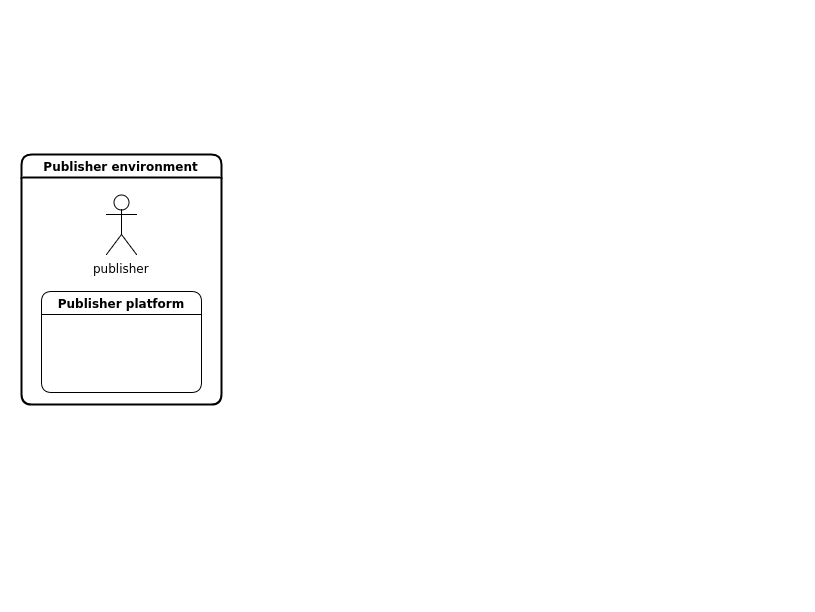
\includegraphics[width=0.9\textwidth]{img/h1}
        \end{frame}

        \begin{frame}{A slice: social media}
            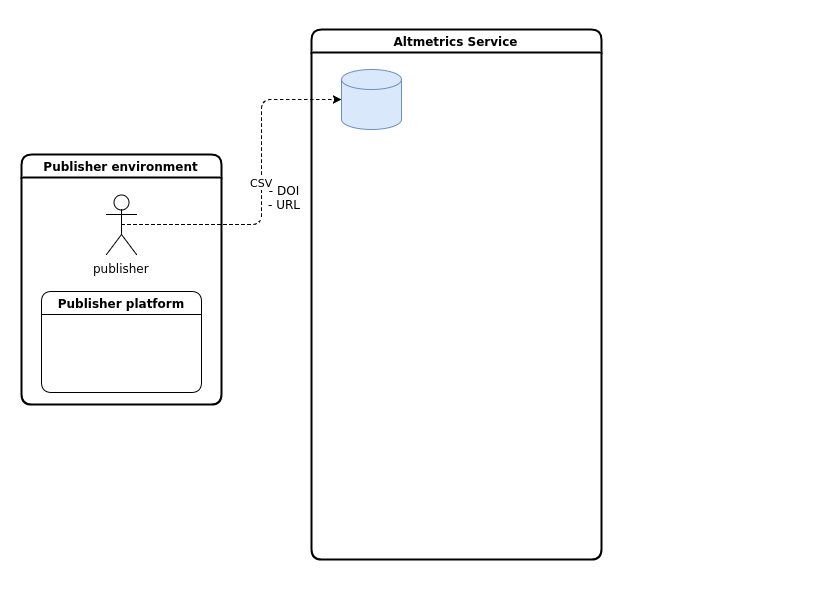
\includegraphics[width=0.9\textwidth]{img/h2}
        \end{frame}

        \begin{frame}{A slice: social media}
            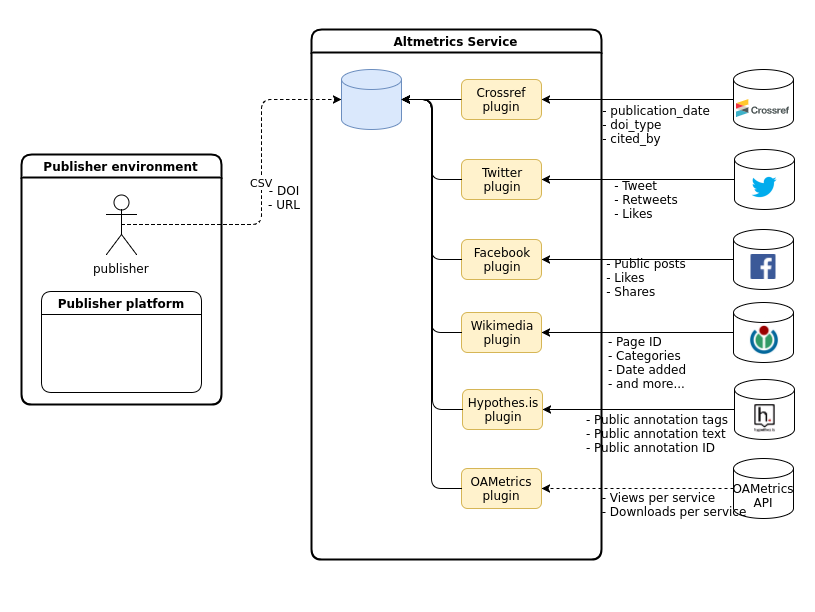
\includegraphics[width=0.9\textwidth]{img/h3}
        \end{frame}

        \begin{frame}{A slice: social media}
            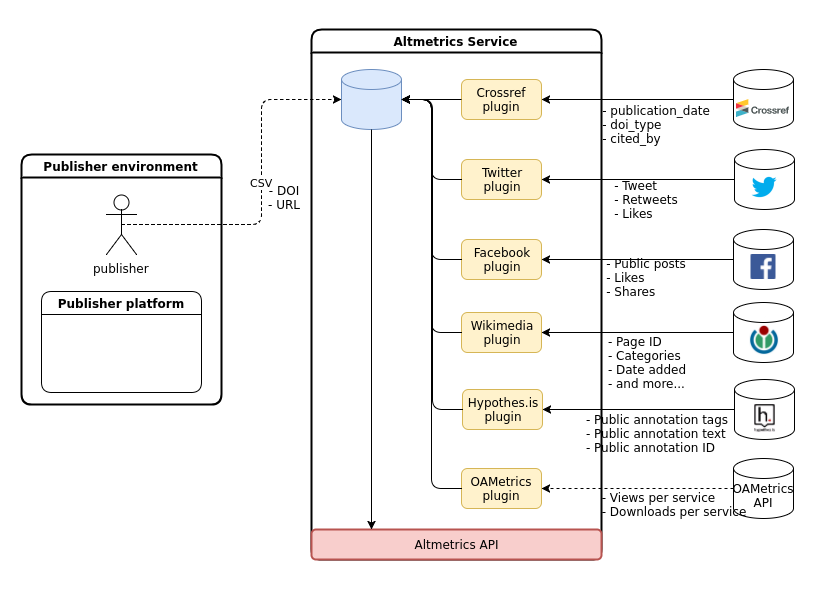
\includegraphics[width=0.9\textwidth]{img/h4}
        \end{frame}

        \begin{frame}{A slice: social media}
            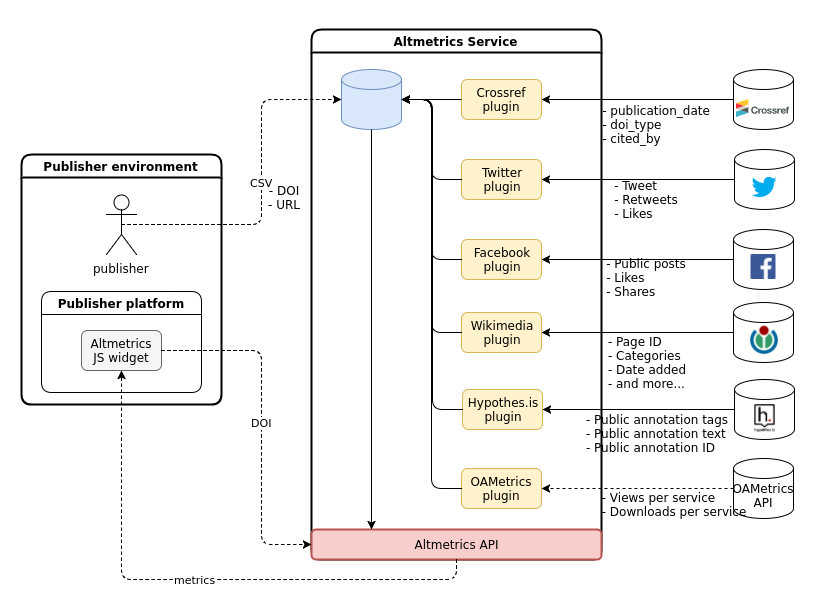
\includegraphics[width=0.9\textwidth]{img/h5}
        \end{frame}

    \subsection{Backend services}

        \begin{frame}{The back-end services: solving the problem}
            Handling publishers' \textbf{private data and credentials}
            \pause
            \begin{description}
                \item [Statistic Collection Agent] Deployed locally on the publisher's infrastructure, collects publisher-specific data (e.g. web access logs) and data from password-protected services (e.g. Google Books) using "drivers"
            \end{description}
            \pause
            \vspace{0.05\textheight}
            \textbf{Different identifiers} across different data sources
            \pause
            \begin{description}
                \item [Identifier Translation Service] Ensures consistency of data across services using different identifiers (e.g. ISBN vs DOI)
            \end{description}
        \end{frame}

    \subsection{A new entry: repositories}

        \begin{frame}{The future: repository metrics}
            \begin{block}{Disclaimer}
                Repositories are not the main focus of the HIRMEOS Metrics
            \end{block}

            \pause

            \begin{center}
                But...
            \end{center}

            \pause

            \begin{itemize}
                \item DOI-based content and \textbf{support for multiple identifiers} allows integration with documents hosted in data repositories
                \pause
                \item \textbf{REST API} to ingest identifiers from the data repository into the HIRMEOS Metrics API
                \pause
                \item use of \textbf{Dublin Core} on public content hosted in data repositories will allow integration
            \end{itemize}
        \end{frame}

        \begin{frame}{The future: repository metrics}
            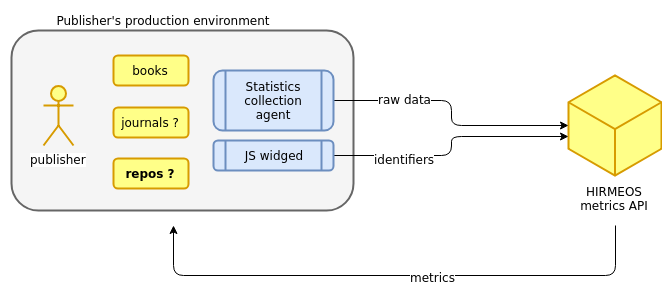
\includegraphics[width=0.9\textwidth]{img/wp6_for_repositories}
        \end{frame}

        \begin{frame}{Give us the good news!}
            \pause
            \begin{center}
                \Huge{End of 2018.}
            \end{center}
            \pause
            \vspace{0.05\textheight}
            \begin{center}
                \Huge{Open source!}
            \end{center}
            \pause
            \vspace{0.05\textheight}
            \begin{center}
                \Huge{https://github.com/hirmeos}
            \end{center}
        \end{frame}

        \begin{frame}{Thanks!}
            \begin{center}
                \Huge{www.hirmeos.eu}
            \end{center}
            \vspace{0.5\textheight}
            \begin{center}
                \Large{francesco.devirgilio@ubiquitypress.com}
            \end{center}
        \end{frame}

\end{document}
